% 
% Annual Cognitive Science Conference
% Sample LaTeX Paper -- Proceedings Format
% 

% Original : Ashwin Ram (ashwin@cc.gatech.edu)       04/01/1994
% Modified : Johanna Moore (jmoore@cs.pitt.edu)      03/17/1995
% Modified : David Noelle (noelle@ucsd.edu)          03/15/1996
% Modified : Pat Langley (langley@cs.stanford.edu)   01/26/1997
% Latex2e corrections by Ramin Charles Nakisa        01/28/1997 
% Modified : Tina Eliassi-Rad (eliassi@cs.wisc.edu)  01/31/1998
% Modified : Trisha Yannuzzi (trisha@ircs.upenn.edu) 12/28/1999 (in process)
% Modified : Mary Ellen Foster (M.E.Foster@ed.ac.uk) 12/11/2000
% Modified : Ken Forbus                              01/23/2004
% Modified : Eli M. Silk (esilk@pitt.edu)            05/24/2005
% Modified : Niels Taatgen (taatgen@cmu.edu)         10/24/2006
% Modified : David Noelle (dnoelle@ucmerced.edu)     11/19/2014
% Modified : Roger Levy (rplevy@mit.edu)             12/31/2018



%% Change "letterpaper" in the following line to "a4paper" if you must.

\documentclass[10pt,letterpaper]{article}

\usepackage{cogsci}

\cogscifinalcopy % Uncomment this line for the final submission 


\usepackage{pslatex}
\usepackage{apacite}
\usepackage{float} % Roger Levy added this and changed figure/table
                   % placement to [H] for conformity to Word template,
                   % though floating tables and figures to top is
                   % still generally recommended!
                   
\usepackage{ifxetex,ifluatex}
\usepackage{microtype}
\makeatletter
\makeatother
\usepackage{xcolor}
\usepackage{xurl}
\usepackage{amsmath} % keep the package, plz

\urlstyle{same} % disable monospaced font for URLs
\usepackage{graphicx}
\usepackage{wrapfig}
\makeatletter
\def\maxwidth{\ifdim\Gin@nat@width>\linewidth\linewidth\else\Gin@nat@width\fi}
\def\maxheight{\ifdim\Gin@nat@height>\textheight\textheight\else\Gin@nat@height\fi}
\makeatother
\setkeys{Gin}{width=\maxwidth,height=\maxheight,keepaspectratio}
% Set default figure placement to htbp
\makeatletter
\def\fps@figure{htbp}
\makeatother
\setlength{\emergencystretch}{3em} % prevent overfull lines
\providecommand{\tightlist}{%
  \setlength{\itemsep}{0pt}\setlength{\parskip}{0pt}}
\setcounter{secnumdepth}{-\maxdimen} % remove section numbering
\ifluatex
  \usepackage{selnolig}  % disable illegal ligatures
\fi

%\usepackage[none]{hyphenat} % Sometimes it can be useful to turn off
%hyphenation for purposes such as spell checking of the resulting
%PDF.  Uncomment this block to turn off hyphenation.

%\setlength\titlebox{4.5cm}
% You can expand the titlebox if you need extra space
% to show all the authors. Please do not make the titlebox
% smaller than 4.5cm (the original size).
%%If you do, we reserve the right to require you to change it back in
%%the camera-ready version, which could interfere with the timely
%%appearance of your paper in the Proceedings.


\title{Statistical Power in Response Signal Paradigm Experiments}
 
\author{{\large \bf Pavel Logačev (pavel.logacev@boun.edu.tr)} \\
  Boğaziçi University - Department of Linguistics \\
  34342 Beşiktaş/İstanbul
  \AND {\large \bf M. İlteriş Bozkurt (ilteris.bozkurt@metu.edu.tr)} \\
  Middle East Technical University - Cognitive Science Department \\
  06800 Çankaya/Ankara}


\begin{document}


\maketitle

\begin{abstract}
Although not widely used, the speed-accuracy tradeoff (SAT) method has produced several prominent findings in sentence processing. While a substantial number of SAT studies has yielded statistical null-results regarding the degree to which certain factors influence the speed of sentence processing operations, the statistical power of the SAT paradigm is not known. As a result, it is not entirely clear how to interpret these findings.
We addressed this problem by means of a simulation study in which we simulated SAT experiments for a range of known effect sizes in order to determine the statistical power in typical SAT experiments.
We found that while SAT experiments appear to have quite satisfactory power to detect differences in asymptotic accuracy, that is not the case for speed-related parameters. We conclude that the failure to find an effect in speed-related parameters in SAT experiments may be less meaningful than previously thought.

\textbf{Keywords:} 
response signal paradigm; speed-accuracy tradeoff; statistical power; simulation
\end{abstract}

\section{Introduction}\label{introduction}

In the field of sentence processing, the speed-accuracy tradeoff method (SAT; e.g., \citeNP{Reed1973,McElree1993}) has been an influential, although not a widely used experimental paradigm.
It addresses the issue that in typical reaction time (RT) tasks involving the processing of sentences or other stimuli, speed and accuracy are related, as many cognitive tasks can be performed more accurately at the cost of lower speed, or faster at the expense of accuracy (e.g., \citeNP{Pachella:1974}). Thus, average RT and accuracy, such as obtained in typical RT tasks, reflect not only the processing speed and accuracy on that task, but also the participant's \textit{response criterion}, i.e., the mechanism by which they determine that they have processed a stimulus to a sufficient degree in order to respond.

% ... accuracy is never perfect and so we can't know that the RT is the processing time ...
Differences between speed-accuracy tradeoff functions (SATF) of two experimental conditions can yield important insights into the cognitive processes that underlie their processing because they make it possible to dissociate the speed of a mental process from its probability of success. For example, \citeA{McElree2000} showed that in the resolution of filler-gap dependencies in sentences like (1), increased distance between the head noun of the relativized noun phrase \textit{'book'} and the verb \textit{'admired'} decreased the probability of successful dependency resolution, but did not affect the processing speed. That is, while participants did quite well at correctly judging grammatical sentences like (1a) and their ungrammatical counterparts like (1a') after a sufficient amount of time, they did not performed as well with sentences like (1b) and (1b'). However, the increase in accuracy relative to this ultimate accuracy(?) was the same in both condition pairs. Because discriminating between grammatical and ungrammatical sentences in (1) arguably requires the retrieval of \textit{book} from working memory, this finding suggests that in sentence comprehension, distance affects the probability of successful retrieval of dependents from memory, but not the speed of the retrieval process.

\setlength{\leftmargini}{3.2em}
\begin{itemize}
\item[(1a/a')] This was the \textit{book} that the editor \textit{admired/*amused}. 
\item[(1b/b')] This was the \textit{book} that the editor who the receptionist married \textit{admired/*amused}.
\end{itemize}

This finding, as well as a number of other results in the SAT literature (e.g., \citeNP{McElree2003,Foraker2007,Martin2008,VanDyke2011}) rest on the absence of a significant difference in speed-related parameters of the speed-accuracy tradeoff function. Because SAT data is typically analyzed using a variant of a \textit{stepwise model selection procedure} 
%(-cite prob machine learning book?-) 
known as \textit{hierarchical model selection} (e.g., \citeNP{Foraker2018}), it is unfortunately not clear how much statistical power such experiments have in order to find differences in processing speed. 
In order to understand how to interpret such statistical null-results, we conducted a simulation study to determine the amount of statistical power in typical SAT experiments.

\section{The Response Signal Paradigm}\label{the-response-signal-paradigm}

In typical sentence processing SAT experiments, participants see sentences of different types, such as in (1), in rapid serial visual presentation (RSVP) and are asked to judge their acceptability after different amounts of time relative to the onset of the last phrase of the sentence. Typically, an auditory cue is used as cue to respond immediately, even if participants have not yet finished making a decision. In the so-called \textit{single-response} paradigm (\textit{SR-SAT}), participants are prompted to respond once per trial. In the \textit{multiple-response} paradigm (\textit{MR-SAT}), respond several times per trial, at different lags (e.g. \cite{McElree1993}).

As in the \citeA{McElree2000} experiment, the experimental design needs to ensure that discrimination between acceptable and unacceptable sentences requires participants to deploy the cognitive process being studied. As a result, the difference between SATFs will (at least partially) reflect the timing of the cognitive process involved -- the number of trials on which the relevant process has terminated will increase with the passage of time, and so will accuracy in both grammatical and ungrammatical conditions.

In order to factor out response bias towards `yes' or `no' responses, the accuracy at each lag in each experimental condition pair is computed as the \textit{Signal Detection Theory (SDT)} sensitivity measure $d' = \Phi(\textit{hits}) - \Phi(\textit{false alarms})$, where $\Phi$ is the Gaussian distribution function, and \textit{hits} and \textit{false alarms} are the proportions of `yes' responses in grammatical and ungrammatical conditions, respectively. The resulting $d'$ values at each lag allow us to estimate the underlying SATF in each experimental condition, which is typically well-approximated by a negatively accelerated shifted exponential function such as in equation \ref{eq:satf} \cite{Dosher1979}. Such an approximation of empirically obtained accuracy estimates is illustrated in Figure \ref{fig:illustrationSATF}. In it, $\lambda$ (\textit{asymptotic accuracy}) determines the highest attainable level of accuracy given unlimited processing time, and $\delta$ (\textit{intercept}) and $\beta$ (\textit{rate}) jointly determine the processing speed: $\delta$ determines at which point the accuracy rises above chance, while $\beta$ determines how quickly the SATF increases. The reciprocal of the rate $\beta^{-1}$ can be interpreted as the time required for the function to reach approximately $63\%$ of the asymptote  (e.g., \citeNP{Liu2009,Foraker2018}).


\begin{equation}
d_t' = \lambda \cdot \left(1-e^{-\beta(t-\delta)} \right),~for~t > \delta;~else~d_t'=0
\label{eq:satf}
\end{equation}

\begin{figure}[t]
\centering
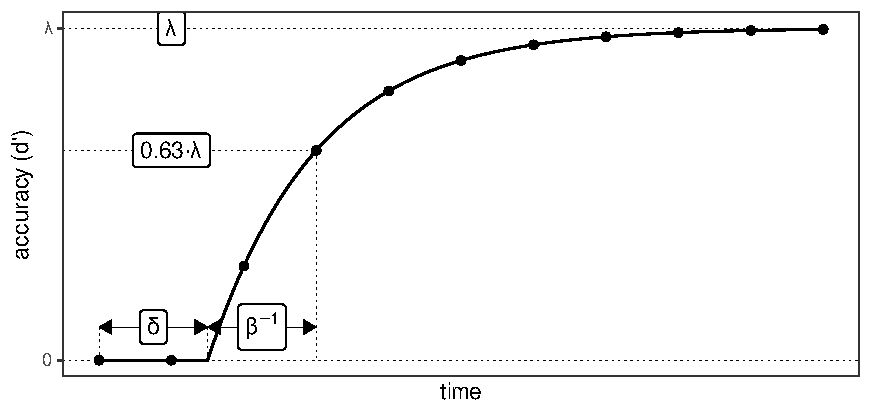
\includegraphics{../figures/illustrations/illustration_satf.pdf} %[width=0.5\textwidth,height=\textheight]
\caption{\label{fig:illustrationSATF}A speed-accuracy tradeoff following equation \ref{eq:satf}. After an initial period of chance performance, accuracy begins to increase at the intercept ($\delta$). The growth rate ($\beta$) determines how quickly the function approaches the asymptotic performance ($\lambda$).
The reciprocal of the rate $\beta^{-1}$ can be interpeted as the time required for the function to reach approximately $63\%$ of the asymptote.
}
\end{figure}


Analysis of data from response signal paradigm experiments follows a variant of a stepwise model selection procedure sometimes referred to as a \textit{hierarchical model testing scheme} (e.g., \citeNP{Foraker2018}):
The aim is to select the most parsimonious of a range of models of varying complexity according to several criteria. For two-condition experiments, there are 8 candidate models. The simplest model (\(1\delta-1\beta-1\lambda\)) posits a single intercept, rate, and asymptote for both experimental conditions. The most complex model (\(2\delta-2\beta-2\lambda\)) posits separate intercepts, rates, and asymptotes for both experimental conditions. Further models of intermediate complexity that are also considered in the process are \(1\delta-1\beta-2\lambda\), \(1\delta-2\beta-1\lambda\), \(1\delta-2\beta-2\lambda\),
\(2\delta-1\beta-1\lambda\), \(2\delta-1\beta-2\lambda\), and
\(2\delta-2\beta-1\lambda\).
Each model corresponds to a particular pattern of differences between experimental conditions: Differences in asymptotes ($\lambda$) can be interpreted as differences in the success probability of the target process, while differences in rate and intercept, jointly considered \textit{the dynamics}, can be interpreted as differences in processing speed.

The parameters for each such model are typically estimated separately for each participant by means of numerical optimization minimizing the \textit{root mean squared error (RMSD)} of the model fit.  \cite{Foraker2018} recommend \textit{forward model selection} starting with the asymptote parameter $\lambda$. As illustrated in Figure \ref{fig:model_selection}A, this process works by successively comparing nested models, beginning with the simplest model \(1\delta-1\beta-1\lambda\) and \(1\delta-1\beta-2\lambda\) in order to determine whether to assume one or two asymptotes. The choice made at this point affects which models will be considered later. If there is sufficient evidence for the two-asymptote model, this means that there is a difference in asymptotes between the two experimental conditions, and only \(2\lambda\) models are considered at later stages; otherwise only \(1\lambda\) models are considered.

Similarly, the choice regarding the number of intercept parameters affects which models are considered at the third stage of the forward model selection procedure, when the number of rates is determined in the example in Figure \ref{fig:model_selection}.

The alternative is \textit{backward model selection}, illustrated in Figure \ref{fig:model_selection}B. In the model selection process, we start with the most complex model \(2\delta-2\beta-2\lambda\), and compare it to increasingly less complex nested models. If no evidence is found for the more complex model, the simpler model is adopted.

Models are compared based on (i) \textit{adjusted \(R^2\)}, which takes into account the fit and penalizes for the number of parameters, and (ii) the consistency of the direction of the difference of the parameter estimates in the more complex models, as assessed by a statistical test.

\begin{figure}[t]
\centering
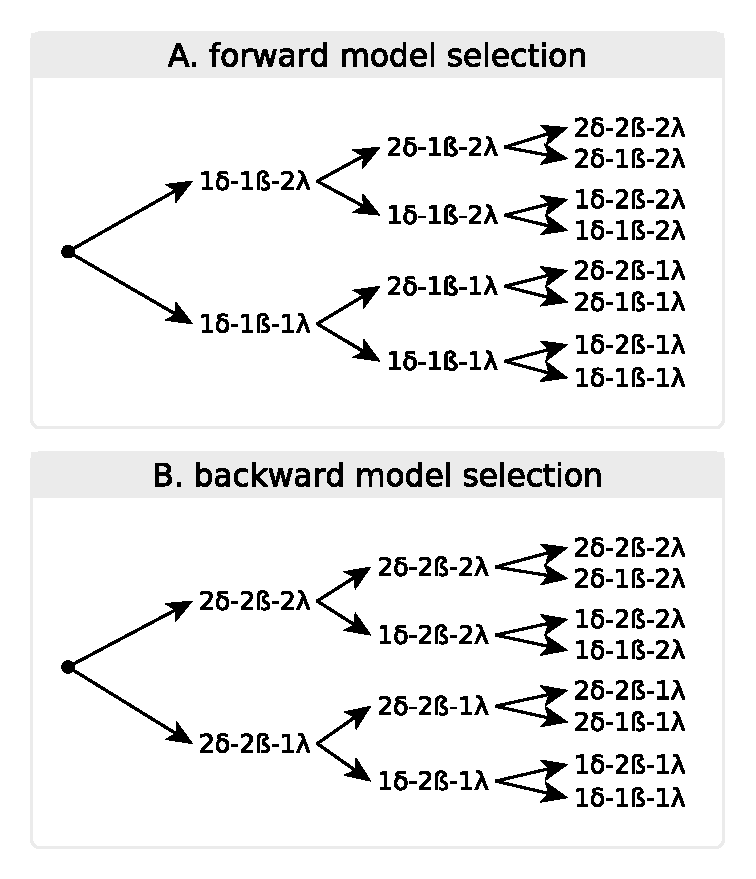
\includegraphics{../figures/illustrations/decision_algo.pdf} %[width=0.5\textwidth,height=\textheight]
\caption{\label{fig:model_selection}Illustration of the forward and backward model selection processes, in which the number of asymptotes is determined first, then the number of intercepts, and then the number of rates.}
\end{figure}

\section{Simulation Study}\label{our-simulations}

In order to determine the statistical power of the stepwise model selection approach typically used in the analysis of SAT experiments, we repeatedly simulated data for a number of different effect sizes in asymptotic accuracy and dynamics, applied this technique to select a model, and compared the results to the known ground truth.

\subsection{Method}\label{method}

We repeatedly simulated SR-SAT and MR-SAT experiments with two experimental condition pairs (two signal conditions, and two noise conditions). Figure \ref{fig:satf_simulation} provides an overview of the process. We assumed that the average population SATF followed equation \ref{eq:satf} with \(\delta=0.8\,sec\), \(\alpha=0.8\,sec\), \(\lambda=2.25\). We further assumed that the individual SATF parameters for each subject \(s\) (\(\lambda_S\), \(\alpha_S\), \(\delta_S\)) were log-normally distributed around the population parameters (\(SD_{\delta}=0.8\), \(SD_{\alpha}=0.8\), \(SD_{\lambda}=1.25\)). We simulated data for a range of differences between conditions in the three SATF population parameters.

% all the deltas were in the the right direction, even though there was a distribution


For each combination of parameters, we simulated \(1,000\) experiments with 20 participants each, and simulated responses at 17 lags starting from \(0\,sec\) to \(5.6\,sec\), increasing in steps of \(0.35\,sec\). We simulated different numbers of responses: \(20\), \(50\), and \(80\) in each of the four experimental conditions for each of the 17 lags. In simulating responses, we assumed that \(P(R_{c,t}=0)\), the probability of a `no' response in condition \(q\) at time \(t\) is given by equation \ref{eq:p_no}. We assumed that responses were equibiased towards `yes' and `no' responses, and that the response criterion $c$ at time $t$ was always $c_t = d_t/2$.  


\begin{equation}
\begin{split}
P(R_{t,q}=0) = \Phi(c_t-\psi_{t,q})\text{, where} \\
\psi_{t,q} =
        \begin{cases}
            d_t & \text{in `yes' conditions} \\
            0 & \text{in `no' conditions}
        \end{cases}
\end{split}
\label{eq:p_no}
\end{equation}


Because in MR-SAT experiments participants respond several times per
trial, it stands to reason that the responses within the trial are
correlated since it appears likely that the amount of evidence in favor
of a particular response at lag \(k\) would at least partially depend on
the amount of evidence available in its favor of that response at lag \(k-1\). We modeled this serial dependence based on assumptions akin
to accumulator models: We assumed that \(\psi'_k\), the amount of
evidence in favor of a `signal' response on any particular trial at lag
\(k\) is normally distributed around \(\psi_k\) with \(\sigma=1\). We
further assumed that \(\psi'_k\) depended on \(\psi'_{k-1}\) as in
equation \ref{eq:mr_sat}.


\begin{equation}
  \psi'_k = \left(1-\frac{1}{\sqrt{k}} \right) \psi'_{k-1} + \frac{1}{\sqrt{k}}\epsilon_k\text{, where }\epsilon_k \in \mathcal{N}(0,1)
\label{eq:mr_sat}
\end{equation}

\begin{figure*}
\centering
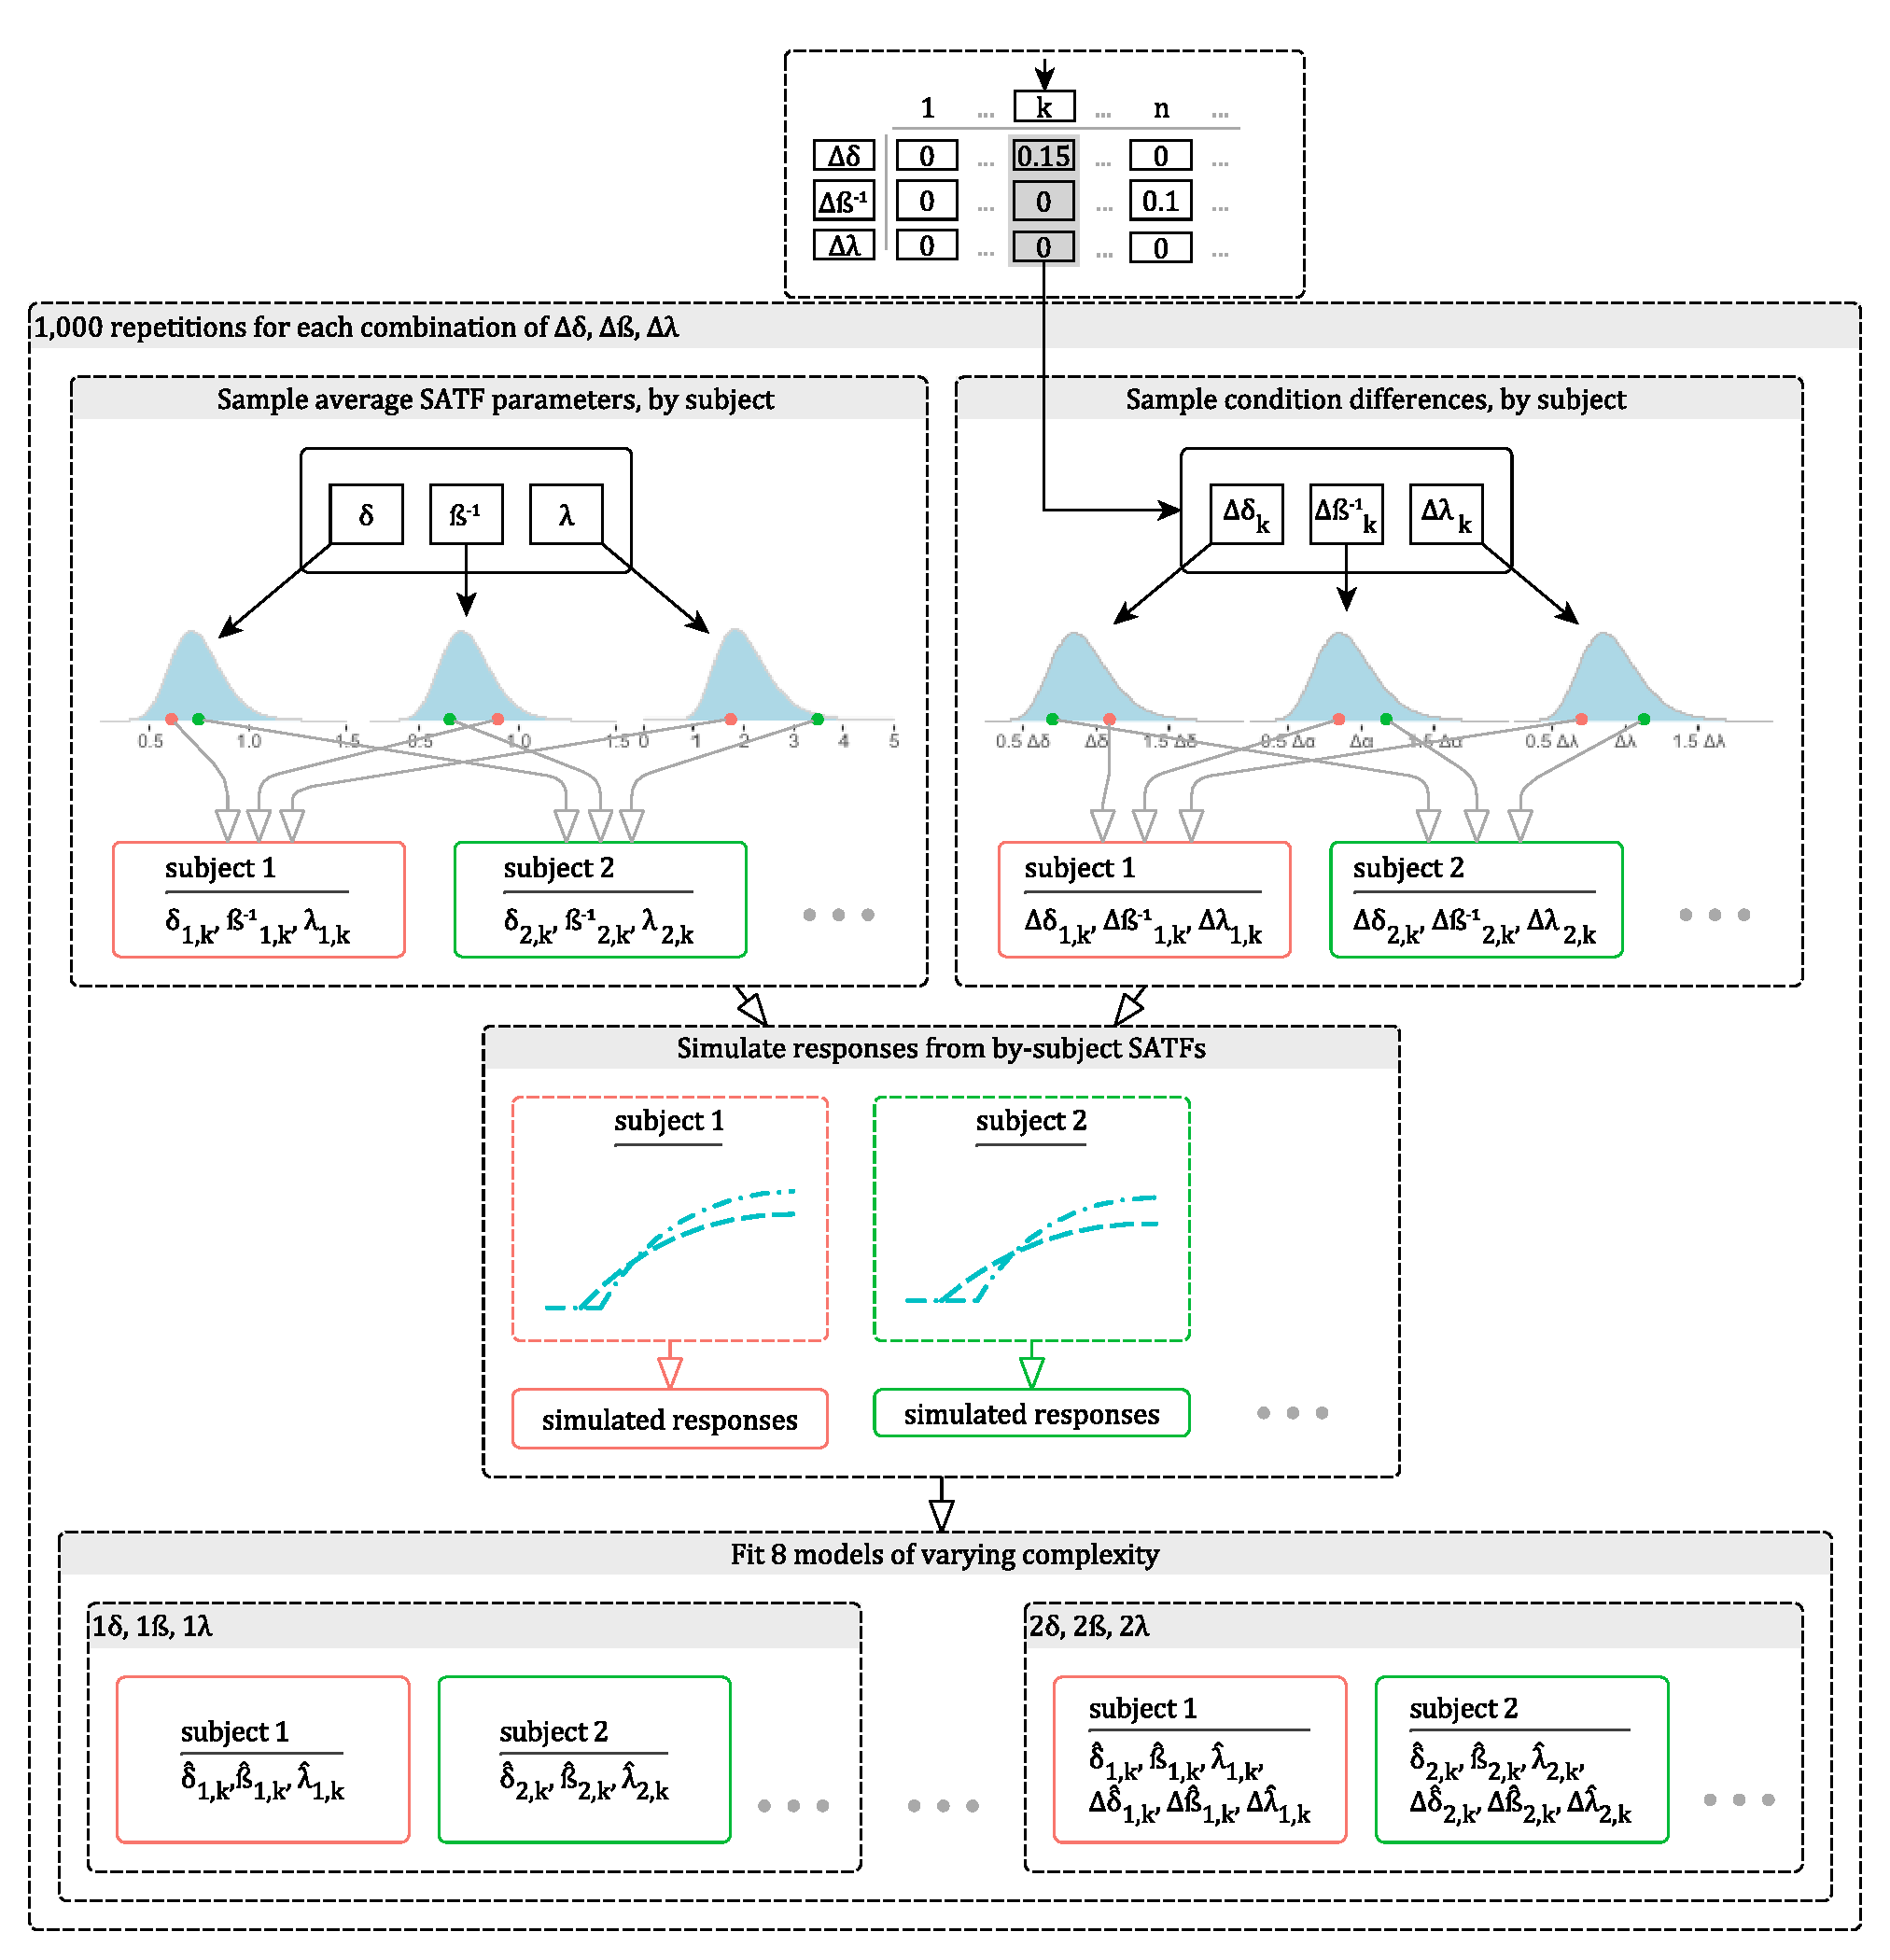
\includegraphics{../figures/illustrations/satf_simulation.pdf} %[width=0.75\textwidth,height=\textheight]
\caption{\label{fig:satf_simulation}Illustration of the simulation process: For each parameter combination for $\Delta\delta$, $\Delta\beta^{-1}$, $\Delta\lambda$, we simulated out $1,000$ experiment with $20$ participants. In each iteration of this process, we independently sampled the by-participant parameters for $\delta$, $\beta^{-1}$, $\lambda$, $\Delta\delta$, $\Delta\beta^{-1}$, and $\Delta\lambda$ from their respective distributions. We then sampled `yes'/`no' responses for each of the 17 lags in each of the 4 conditions, computed $d'$ at each lag, for each condition pair for each simulated participant, fitted several models of varying complexity to each participants data, and carried out model comparison for each simulated experiment. Simulations SR-SAT and MR-SAT were carried out independently.  }
\end{figure*}

\subsection{Analysis}\label{analysis}

We used \textit{R} (\citeNP{R-base}) and the \textit{tidyverse} packages (\citeNP{R-tidyverse}) for simulation and data pre-processing, and the \textit{mrsat} R package (\citeNP{VanDykeEtAl:2015}) to fit eight models of varying degrees of complexity to each simulated participant's data.

We used five different model selection procedures on each of the simulated experiments:
As a baseline analysis method, we tested for significant differences between estimates of $\hat{\delta}$, $\hat{\beta}$, $\hat{\lambda}$ in the two conditions based on $2\delta-2\beta-2\lambda$ model estimates.
Moreover, we carried out backward and forward model selection using two sets of criteria:
The first method was model selection based on the results of a t-test on the parameter difference estimates ($\hat{\Delta\delta}$, $\hat{\Delta\beta}$, $\hat{\Delta\lambda}$) of the more complex model. For example, in forward model selection as illustrated in fig. \ref{fig:model_selection}A, we selected model $1\delta-1\beta-2\lambda$ if the estimates of $\Delta\lambda$ significantly differed from $0$, or in other words: if there was a significant different the asymptote estimates of the two experimental conditions. Otherwise, we selected the simpler model $1\delta-1\beta-1\lambda$.
Because \cite{Foraker2018} suggest the use of the \textit{adjusted $R^2$} metric to supplement hypothesis tests, we also tested a more conservative method, in which the more complex model was only selected if its average \textit{adjusted $R^2$} across participants was higher than that of the simpler model, in addition to the relevant parameter difference being significantly different from $0$.
%Moreover: 
%- AIC/BIC (with that group BIC approach I explain in an early draft of the SAT paper)

\begin{figure*}
\centering
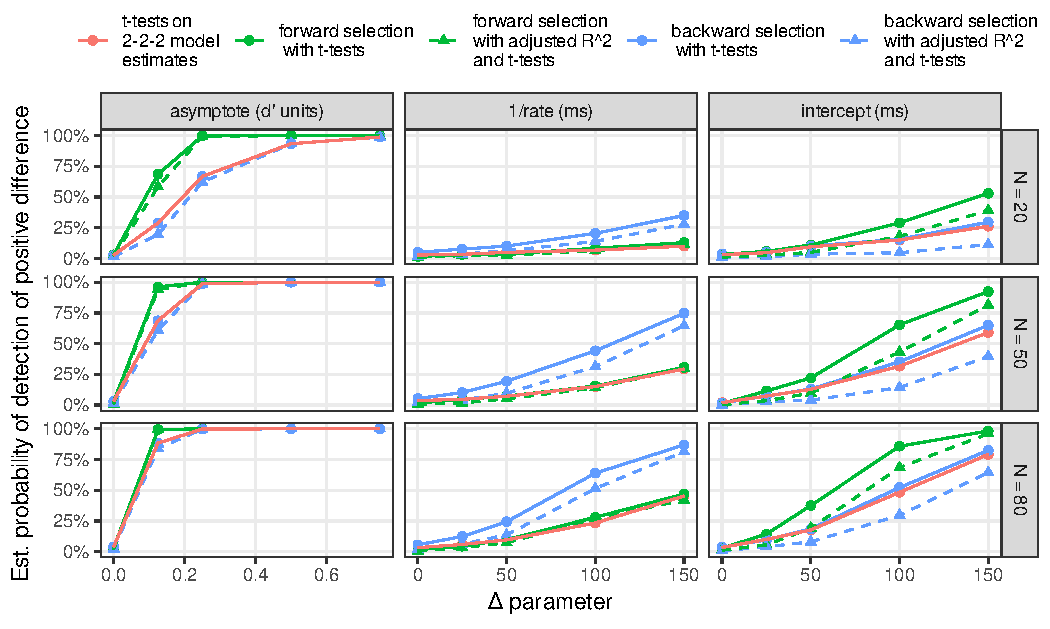
\includegraphics[width=0.75\textwidth]{../figures/results/results_sr.pdf} %[width=0.50\textwidth,height=\textheight]
\caption{\label{fig:res_sr}Simulation results for \textit{single-response SAT}: For each of the three SATF parameters (columns), the x-axis the represents the magnitude of the population difference, while the y-axis corresponds to the proportion of simulated experiments in which the selected model assumed a positive value for the respective difference \protect{$\Delta\lambda$} (left), \protect{$\Delta\beta^{-1}$} (center), \protect{$\Delta\delta$} (right). Rows represent simulations with different numbers of responses per condition (4) per lag (17). Each point based on the simulation of $1,000$ experiments with 20 participants. }
\end{figure*}

\begin{figure*}
\centering
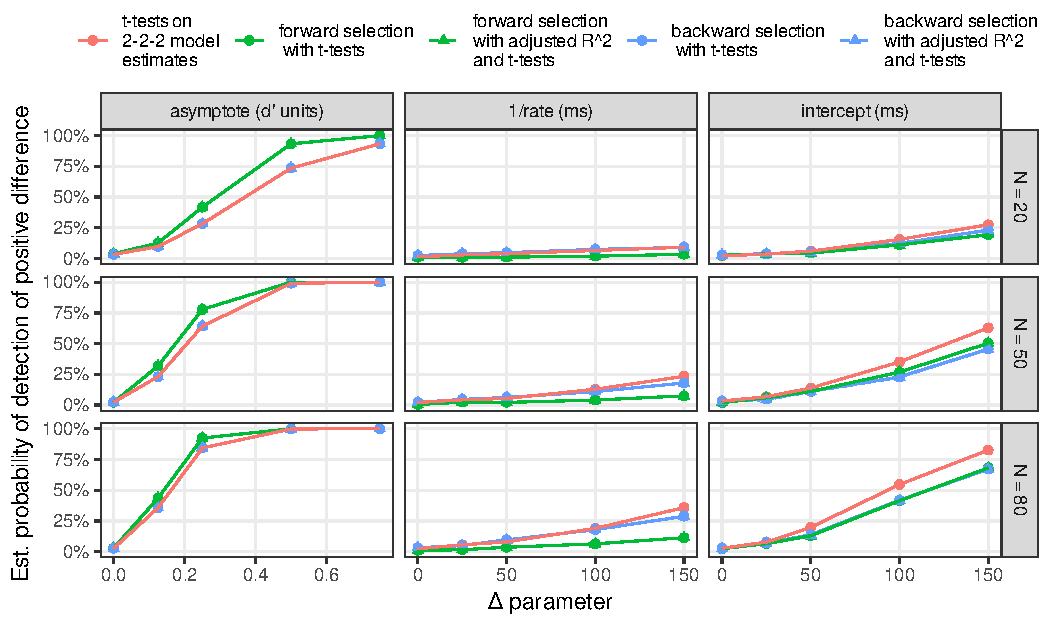
\includegraphics[width=0.75\textwidth]{../figures/results/results_mr.pdf} %[width=0.50\textwidth,height=\textheight]
\caption{\label{fig:res_mr}Simulation results for \textit{multiple-response SAT}: For each of the three SATF parameters (columns), the x-axis the represents the magnitude of the population difference, while the y-axis corresponds to the proportion of simulated experiments in which the selected model assumed a positive value for the respective difference \protect{$\Delta\lambda$} (left), \protect{$\Delta\beta^{-1}$} (center), \protect{$\Delta\delta$} (right). Rows represent simulations with different numbers of responses per condition (4) per lag (17). Each point based on the simulation of $1,000$ experiments with 20 participants. }
\end{figure*}

\section{Results \& Conclusion}\label{results}

Figures \ref{fig:res_sr} and \ref{fig:res_mr} show the results of our simulations. They show that all model selection methods have reasonably high power ($>80\%$) to detect an asymptote difference of more than $0.5$ d' units. While for small effect sizes, power is generally higher for the SR-SAT paradigm, it is relatively high overall and largely independent of the model selection method, 
%which is likely due to the fact that asymptotes are considered first 
even for small samples with 20 responses per lag for each participant.

This pattern is quite different from the results concerning the intercept and the rate: SR-SAT and MR-SAT seem to exhibit substantial differences in terms of power in detecting a difference in rates and intercepts, with remarkably low power especially for rate parameter differences of less than $40\%$ even for relatively large effect sizes such as $150\,ms$, and less than $20\%$ in most cases.  
In SR-SAT, the model selection procedure appears to play a significant role in the detection of differences, and it appears that backward model selection based on simple t-tests testing for parameter differences may be the most robust model selection procedure, since, across parameters, it is not consistently outperformed by any other method, and as it appears to usually produce results which are as good as those of the best method. It remains to be seen if this method will be outperformed by a model selection method which compares all models with each other instead of proceeding in a stepwise manner.

Importantly, our findings suggest that the statistical power in typical SAT experiments is relatively low for typical effect sizes in psycholinguistics ($50-100\,ms$), especially when it comes to the intercept and rate parameters. This is even more pronounced for multiple-response SAT experiments. As a result, the failure to find a difference in intercept and rate between two experimental condition pairs should not be interpreted as the absence of an effect.


%\newpage
%\section{Conclusions}\label{conclusions}

%\section{Optional}\label{optional}
%\begin{itemize}
%\tightlist
%\item
%  Do not use this, but keep note of it:
%  Adjusted R2 is a bit of a weird metric because a unit of d' doesn't
%  really mean the same thing at d=0-1 (around the intercept), and at
%  d'=3 (around the asymptote). So the points around the asymptote, and
%  at the late increasing stage may have an undue influence. That's
%  especially problematic, since they are many.
%\end{itemize}

\bibliographystyle{apacite}

\setlength{\bibleftmargin}{.125in}
\setlength{\bibindent}{-\bibleftmargin}

\bibliography{references}


% \section{Appendix}\label{appendix}
% 
% 
% We used the Bayesian information criterion (BIC) for model selection and the BIC approximation to the Bayes factor for inference \cite{Wagenmakers:2007}. The BIC was computed according to equation \ref{eq:BIC}, where $log~L$ is the maximized log-likelihood of the data under a given model, $n_{par}$ is the number of free parameters in the model, and $n_{obs}$ is the number of observations.
% The BIC decreases with increasing log-likelihood of the data and increases with the number of free parameters. The amount of free parameter penalty depends on the amount of data ($n_{obs}$). The model with the smallest BIC provides the most parsimonious fit to the data, and maximizes the generalizability of a model \cite{PittMyung:2002}. Because the responses on one trial were highly correlated, we set $n_{obs}$ to the number of trials for one participant, instead of the actual number of data points.
% 
% 
% \begin{equation}
% \label{eq:BIC}
% BIC = -2\cdot log~L + log(n_{obs})\cdot n_{par}
% \end{equation}
% 
% For formal inference, we used the BIC approximation to the Bayes factor according to equation \ref{eq:BF} \cite{Wagenmakers:2007}, where $BIC_{1}$ and $BIC_{2}$ are the BIC values of the models to be compared. The Bayes factor quantifies the evidence in favor of model 1 over model 2. We combined individual participants' Bayes factors for each comparison into group Bayes factors (GBF) as well as average Bayes factors (ABF), as suggested by \citeA{StephanPenny:2006}. The GBF for comparison of models 1 and 2 was computed according to equation \ref{eq:GBF} as the product of all participants' Bayes factors for that comparison (where $k$ is an index over participants).
% Like a single Bayes factor, a GBF can be interpreted as the ratio of evidence in favor of model 1 and the evidence in favor of model 2. By convention (e.g., Raftery:1995), the evidence is considered \textit{weak} when $1 < BF < 3$, \textit{positive} when $3 < BF < 20$, \textit{strong} when $20 < BF < 150$, and \textit{very strong} positive when $BF > 150$. We chose to present $log$ GBFs ($l$GBFs) here because the value of the GBF tended to become rather large. On a log scale, values above $1$ can be considered positive evidence, and a values above $3$ and $5$, respectively, can be considered \textit{strong} and \textit{very strong} evidence.
% %\TODO{ Read Raftey(1995), which explains this approximation in more detail. Copy is in the literature folder.}
% 
% 
% \begin{equation}
% \label{eq:BF}
% BF_{12} = e^{(BIC_{2} - BIC_{1})/2 }
% \end{equation}
% 
% \begin{equation}
% \label{eq:GBF}
% GBF_{12} = \prod_{k}{ BF_{12(k)} }
% \end{equation}
% 
% 
% To complement the GBF, \citeA{StephanPenny:2006} suggest providing an average Bayes factor (ABF), which is the geometric mean of the individual Bayes factors (and therefore $ABF_{12} = \sqrt[N]{GBF_{12}}$, where $N$ is number of participants). In contrast to the GBF, the ABF is not dependent on the number of participants and can thus be more easily compared across different experiments. It can be interpreted as the average participant-level Bayes factor contributing to the GBF.
% 
% We used the Bayes factor-based comparisons for models with constrained differences between asymptotes and intercepts. We supplement these comparisons with the analysis of coefficient estimates from unconstrained fully saturated models.





\end{document}